\chapter{Конструкторский раздел}
\label{cha:design}

В данном разделе будут рассмотрены схемы алгоритмов и структура реализации.

\section{Схемы алгоритмов сортировки}
На рисунке ~\ref{fig:radix_sort} приведена схема алгоритма поразрядной сортировки.
На рисунке ~\ref{fig:heap_sort} приведена схема пирамидальной сортировки.
На рисунке ~\ref{fig:bubble_sort} приведена схема пузырькового алгоритма сортировки.

\begin{figure}
    \centering
    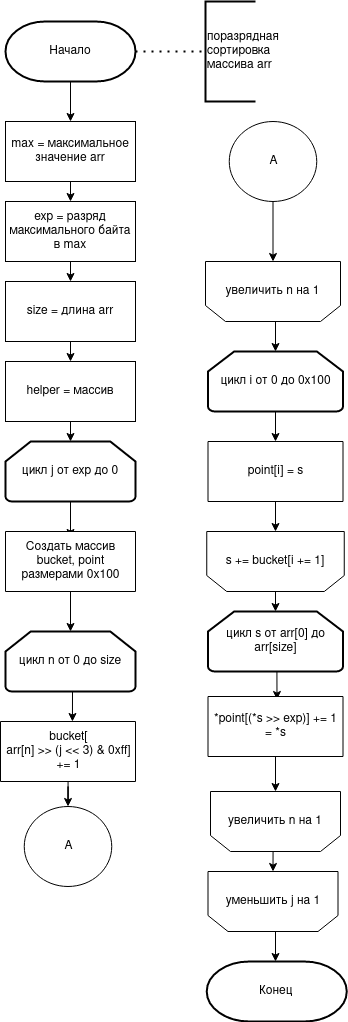
\includegraphics[height=0.75\textheight]{sem-v-aa-master/lab1/tex/inc/schemes/radix_sort.png}
    \caption{Схема алгоритма поразрядной сортировки}
    \label{fig:radix_sort}
\end{figure}

\begin{figure}
    \centering
    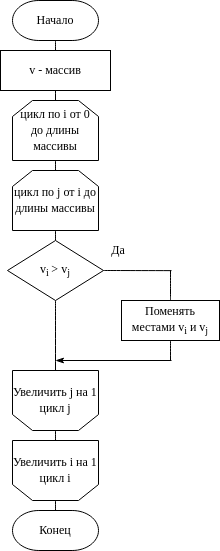
\includegraphics[height=0.75\textheight]{sem-v-aa-master/lab1/tex/inc/schemes/bubble_sort.png}
    \caption{Схема алгоритма пузырьковой сортировки}
    \label{fig:bubble_sort}
\end{figure}

\begin{figure}
    \centering
    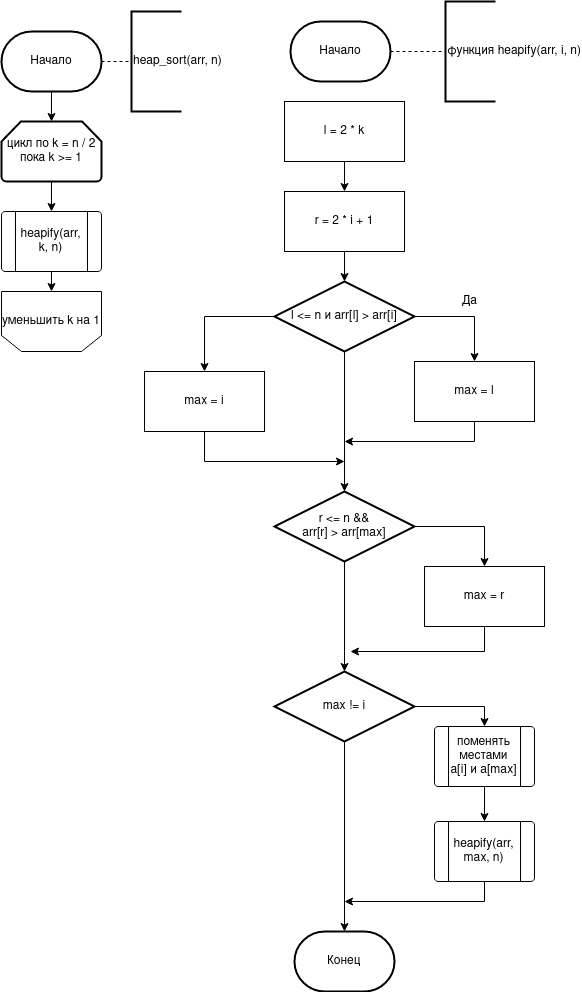
\includegraphics[height=0.75\textheight]{sem-v-aa-master/lab1/tex/inc/schemes/heap_sort.png}
    \caption{Схема алгоритма пирмаидальной сортировки}
    \label{fig:heap_sort}
\end{figure}

\section{Модель вычислений} 
Для последующего вычисления трудоемкости введем модель вычислений:
\begin{enumerate}[1.]
    \item Операции из списка \ref{eq:operations} имеют трудоемкость $1$. 
    \begin{equation}
        +,-,/,\%,=,\ne,<,>,\leq,\geq,[\;],++,--
        \label{operations}
    \end{equation}
    \item Трудоемкость условного оператора расчитвыается как \ref{eq:conditional}
    \begin{equation}
        f_{if} = f_{условия} + 
        \begin{cases}
            f_{A},& \text{если условие выполняется},\\
            f_{B},& \text{иначе}.
        \end{cases}
        \label{eq:conditional}
    \end{equation}
    \item Трудоемкость цикла рассчитывается как \ref{eq:loop}
    \begin{equation}
        f_{\text{цикл}} = f_{\text{сравнения}} + N \cdot (f_{\text{тела}} + f_{\text{инкремента}} + f_{\text{сравнения}})
        \label{eq:loop}
    \end{equation}
    \item трудоемкость вызова функции равно $0$.
\end{enumerate}

\section{Трудоемкость алгоритмов}
Пусть размер массив будет обозначаться как $N$.
\subsection{Алгоритм сортировки пузырьком}

Трудоемкость алгоритма сортировки пузырьком состоит из:
\begin{itemize}
    \item трудоемкость сравнения и инкремента внешнего цикла $i \in [1\dots N)$ \ref{eq:outer_loop} \begin{equation}
        f_i = 2 + 2(N - 1)
        \label{eq:outer_loop}
    \end{equation}
    суммарная трудоескость внутренних циклов, количество итераций которых меняется в промежутке $[2\dots N - 1]$ \ref{eq:inner_loop} \begin{equation}
        f_j = 3(N - 1) + \dfrac{N^2 - N}{2} \cdot(3 + f_{ij})
        \label{eq:inner_loop}
    \end{equation}
    \item трудоемкость условия во внутреннем цикле \ref{eq:inner_condition} \begin{equation}
        f_{ij} = 4 +         
        \begin{cases}
            0, & \text{в лучшем случае},\\
            9,& \text{в худшем случае}.
        \end{cases}
        \label{eq:inner_condition}
    \end{equation}
\end{itemize}

Трудоемкость в лучшем случае \ref{eq:bubble_best}
\begin{equation}
    f_{\text{best}} = \frac{7}{2}N^2 + \frac{3}{2}N - 3 \approx \frac{7}{2}N^2 = O(N^2)
    \label{eq:bubble_best}
\end{equation}
Трудоемкость в худшем случае \ref{eq:bubble_worst}
\begin{equation}
    f_{\text{worst}} = 8N^2 + 8N - 3 \approx 8N^2 = O(N^2)
    \label{eq:bubble_worst}
\end{equation}

\subsection{Алгоритм пирамидальной сортировки}

Алгоритм пирамидальной сортировки начинается с построения кучи Build-Max-Heap:

Трудоемкость сравнения и инкремента внешнего цикла $i \in [1..N / 2)$
\begin{equation}
    f_i = 2 + 2(N - 1)
    \label{eq:heap_outer}
\end{equation}

Трудоемкость внутренного цикла, вызванного рекурсивно \ref{eq:heap_inner}, учитывая, что в среднем, длина поддерева будет равна $2/3n$:
    
\begin{equation}
    T(n) \leq T(2n/3) + O(1)
    \label{eq:heap_inner}
\end{equation}

Это можно свести к $O(\log n)$, пользуясь теоремой о рекурентных соотношений \cite{intro_to_algo_heap}.

\subsection{Алгоритм поразрядной сортировки}
Пусть даны N чисел, имеющих разрядность $b$ и любое положительное целое число $r < b$.

Для люого $r \leq b$ мы рассматриваем ключ, имеющим $d = [ b / r ]$ цифр по $r$ бит каждая. Каждая цифра лежит в диапазоне от $0$ до $2^{r} - 1$. В таком случае мы можем использовать сортировку подсчетом с значением $k = 2^r - 1$. Каждый проход сортировки подсчетом займет $O(n + k) = O(n + 2^r)$, а проходов всего --- $d$. Получаем время сортировки $O(d(n + 2^r)) = O((b/r)(n + 2^r))$ \cite{intro_to_algo_radix}.

\subsection{Структуры данных}

В реализации алгоритма пирамидальной сортировки было использовано бинаное дерево. В реализации поразрядной сортировки использовалась карманная сортировка, где использовались несколько массивов (коллекций), в которых содержались значения разрядов ключей массива.

\section{Тестирование}
Тестирование будет проведено на трех классах эквивалентности: заранее отсортированном массиве (в порядке возратания), заранее отсортированном массиве (в порядке убывания) и случайно сформированном массиве.


\section{Вывод}

На основе теоретического материала из аналитического раздела были построены схемы реализаций исследуемых алгоритмов.

%%% Local Variables:
%%% mode: latex
%%% TeX-master: "rpz"
%%% End:
